\documentclass[11pt]{article}

\usepackage[review]{acl}
\usepackage{times}
\usepackage{latexsym}
\usepackage[T1]{fontenc}
\usepackage[utf8]{inputenc}
\usepackage{microtype}
\usepackage{inconsolata}
\usepackage{graphicx}
\usepackage{booktabs}
\usepackage{amsmath}
\usepackage{amssymb}
\usepackage{enumitem}
\usepackage{xcolor}

\title{MUG-Serve: An Inspectable, Latency-Aware Service for\\Retrieval-Gated Medical Question Answering}

\author{Anonymous ACL submission}

\begin{document}
\maketitle

\begin{abstract}
Retrieved passages can pull a strong LLM away from a correct medical answer.
Marginal-utility gating (MUG) admits evidence only when it \emph{moves} the
answer. We present \textbf{MUG-Serve}, an open-source FastAPI/React system that
makes this decision interactive and inspectable. A user asks a multiple-choice or
open-ended medical question; MUG-Serve builds an evidence pool from a textbook
index and live PubMed, runs one of five policies, and streams a span-level trace
of what was retrieved, whether it changed the answer, what was kept or withheld,
and what each step cost. A replay mode shows three recorded cases with no
credentials or network. To audit an existing RAG system, a developer can send its
generation calls, with the retrieved documents in a non-standard field, through
an OpenAI-style proxy (whose \emph{shadow} mode labels requests but returns
plain RAG under MUG-Serve's own prompt), or audit a
frozen JSONL pool in batch. On a live hybrid pool, running the gate's two probes
in parallel cuts its paired median latency by $16$--$20\%$ relative to running
them serially. Under the original study's pool protocol (\texttt{gpt-4o-mini},
$n{=}200$ per dataset), the flip gate's accuracy differs from naive RAG's by
$+0.5$ (MedQA) and $+1.5$ (PubMedQA) points, with paired 95\% CIs that include
zero, while placing $5$--$9\%$ of naive's evidence tokens in the final prompt.
Serving also exposes failures: with \texttt{claude-haiku-4.5} the gate falls
$5$ points below closed-book on MedQA ($p{=}0.04$, uncorrected), live PubMed retrieves the source paper
for $66$ of $150$ PubMedQA questions, and a cheap-scout cascade is matched by a
hindsight router that reads only the question format.
\end{abstract}

\begin{figure*}[t]
\centering
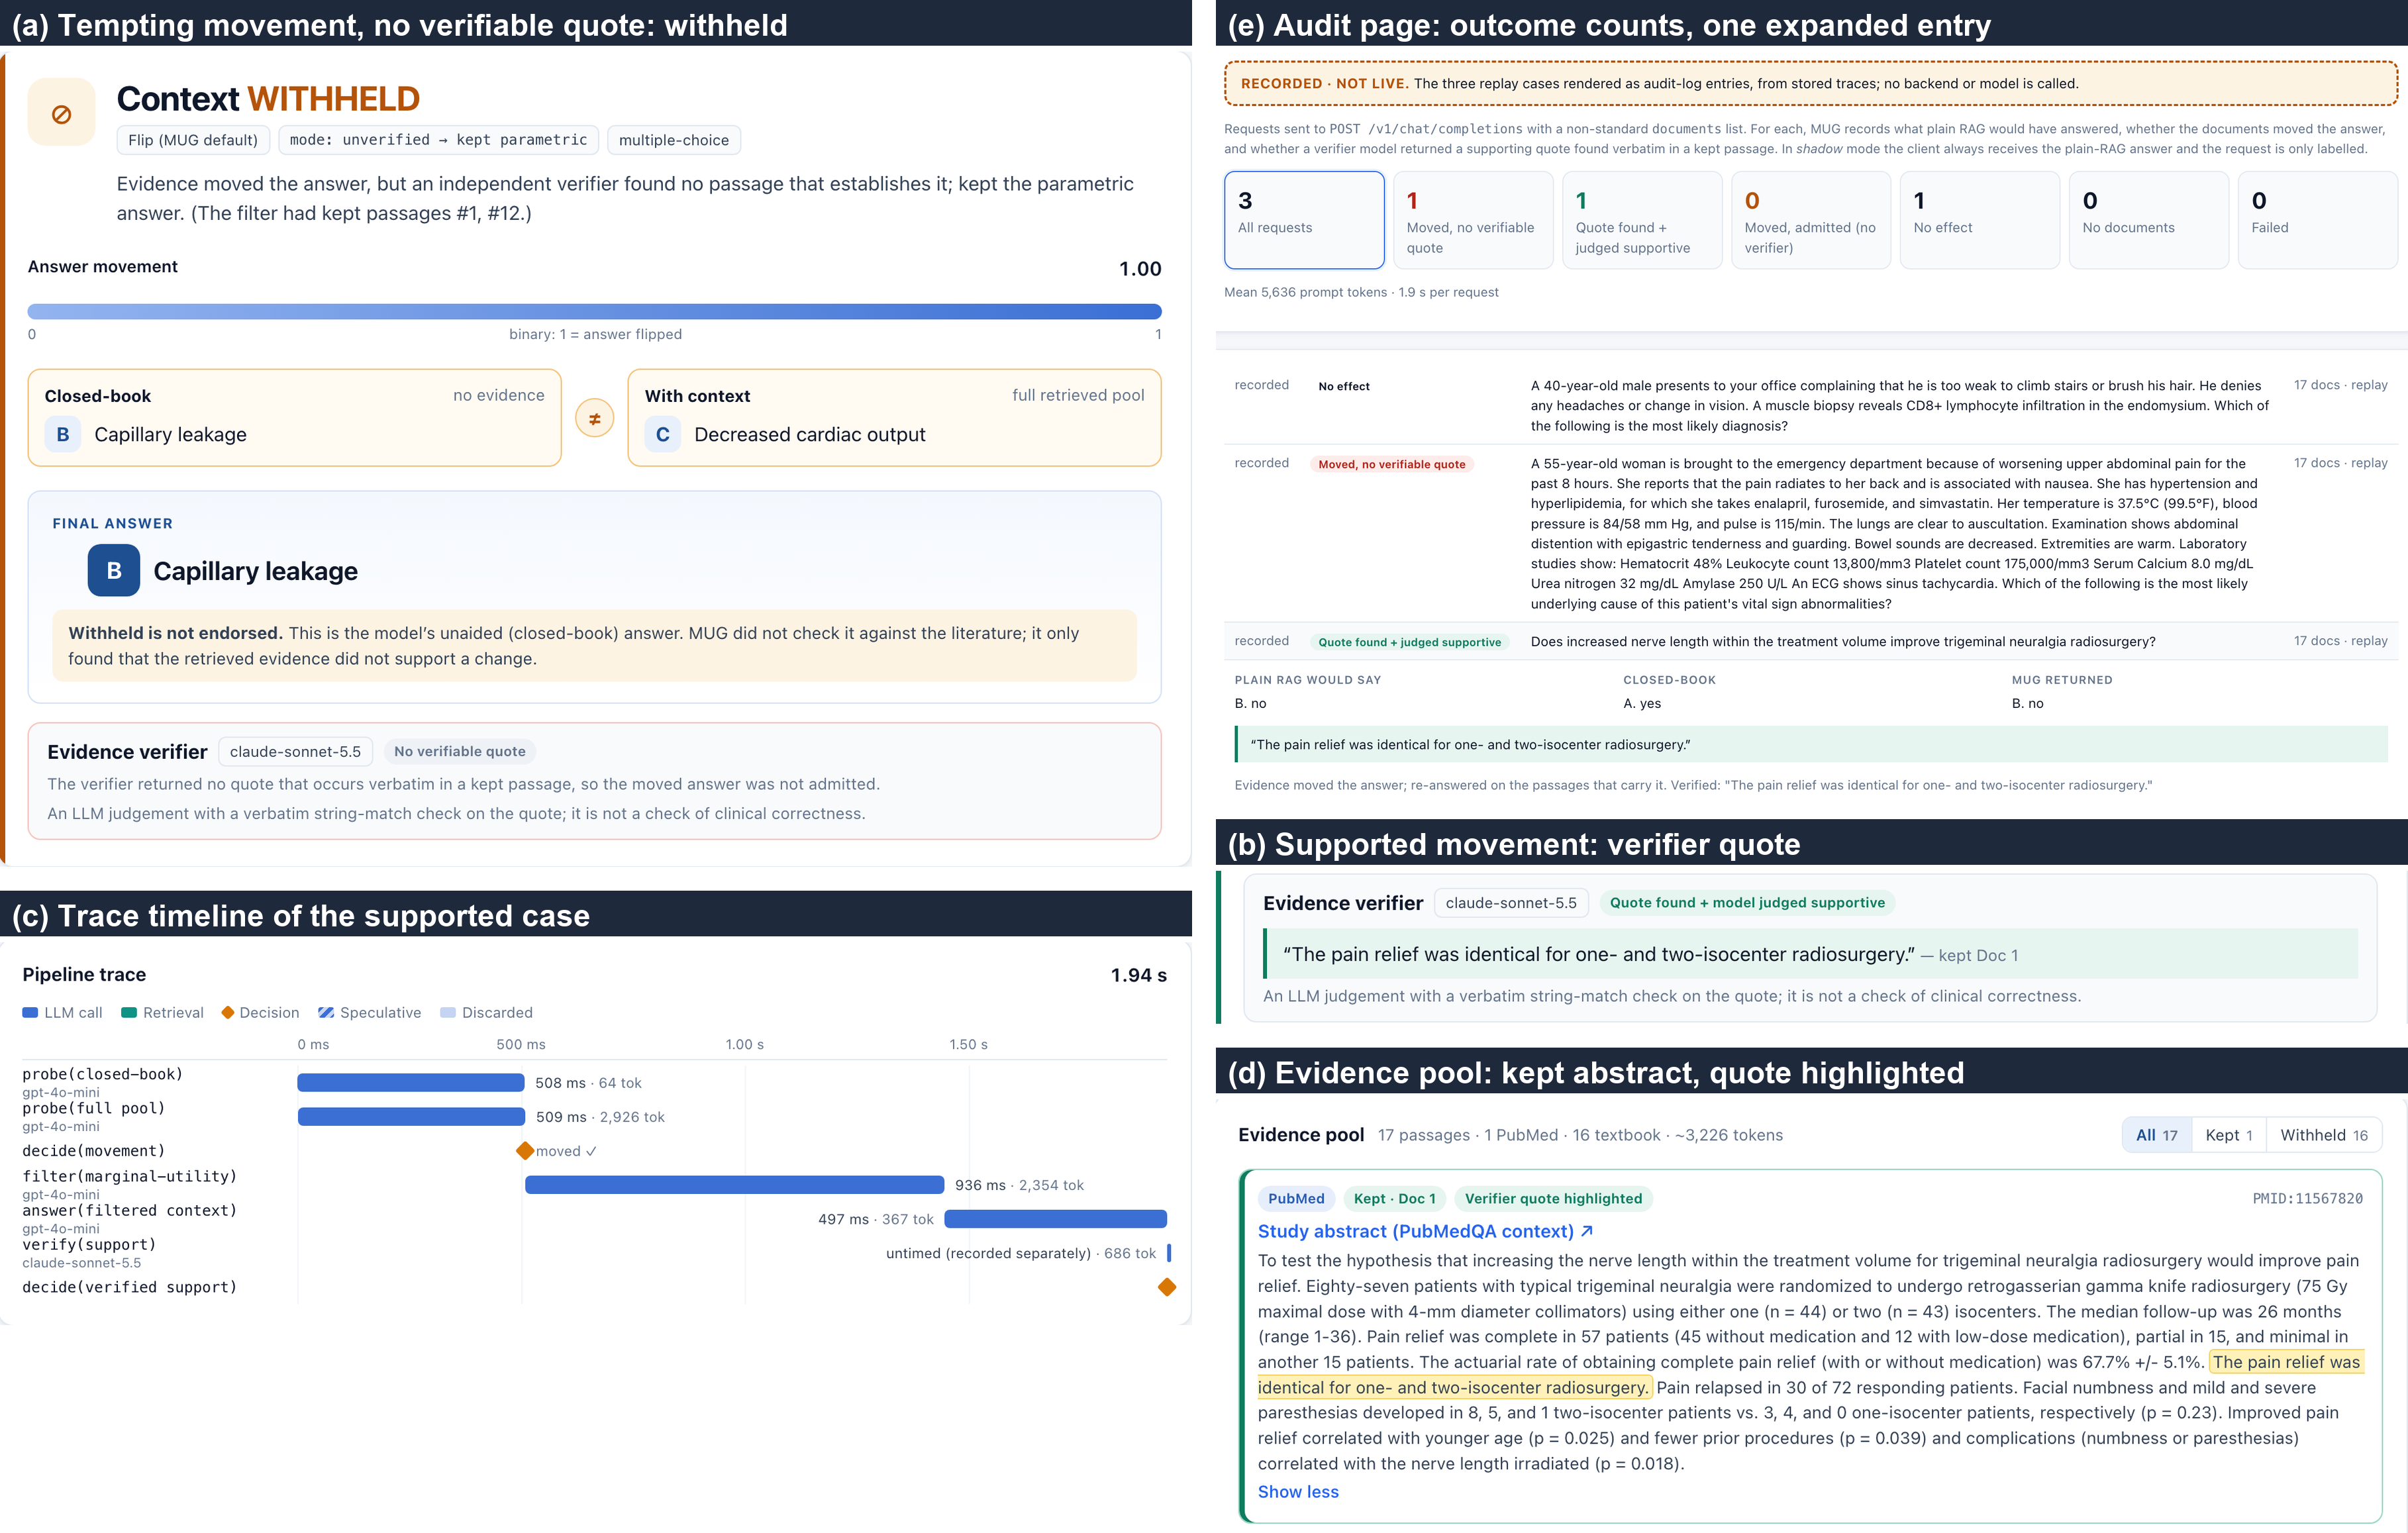
\includegraphics[width=\textwidth]{figs/fig1_composite.png}
\caption{MUG-Serve in Replay mode (recorded cases; no model or network calls).
(a)~MedQA case: the 17-passage pool flips a correct closed-book answer (B) to a
wrong one (C); the verifier returns no quote found verbatim in the kept
passages, so the evidence is withheld and the card states that
\emph{withheld is not endorsed}. (b)--(d)~PubMedQA case: the study abstract
flips a wrong answer to the right one; (b)~the verifier's quote, (c)~the span
timeline (parallel probes, movement decision, filter, re-answer, verifier), and
(d)~the evidence pool with the one kept passage and the quote highlighted (16
withheld passages below, cropped). (e)~The Audit page with per-outcome counts
and one expanded entry.}
\label{fig:ui}
\end{figure*}

% ===========================================================================
\section{Introduction}
% ===========================================================================
Retrieval-augmented generation (RAG)~\citep{rag} is the default way to ground LLM
answers. In medicine it is also a hazard: a strong model's parametric answer is
often right, and plausible but off-target passages can pull it away from that
answer~\citep{distracted,knowledgeconflict,medrag}. Marginal-utility gating
(MUG; \citealp{mug}) puts evidence into the answer window only when the evidence
changes the answer. Serving such a gate raises questions an offline benchmark
does not: it issues $2$--$3$ LLM calls instead of one, many API models lack
log-probabilities, clinicians give no answer options, live search results are
not curated pools, and users need to see \emph{why} an answer was given.
MUG-Serve supports three uses:

\begin{itemize}[leftmargin=1.2em,itemsep=1pt,topsep=2pt]
\item \textbf{Ask and inspect.} A user asks a question and watches it execute:
retrieval, the two probes, the gate decision with a plain-language reason, the
passages kept or withheld, the verifier's quote, and the cost
(Fig.~\ref{fig:ui}). \emph{Compare} runs all five policies on one question.
\item \textbf{Replay.} Three recorded cases render in the same UI without
credentials or network.
\item \textbf{Audit supplied documents.} A proxy, or a batch command on a
frozen JSONL file, records whether the caller's documents moved the answer
under MUG-Serve's own prompt, and whether a verifier found a supporting quote.
\end{itemize}

\noindent Our contributions are (i) the system: movement estimators for models
with and without log-probabilities (including \emph{semantic movement} for
open-ended answers), a hybrid textbook/PubMed pool, a streamed trace UI with a
replay mode, an optional cross-model evidence verifier, and the audit proxy and
batch auditor (\S\ref{sec:system}--\S\ref{sec:demo}); (ii) \emph{latency-aware
scheduling} of the gate's request DAG, with measured latency and token costs
(\S\ref{sec:eval-sched}); and (iii) measurements through the code path a user
exercises, including negative results (\S\ref{sec:eval}). The method~\citep{mug}
and the verifier's evaluation~\citep{influence} are not contributions here.

\smallskip\noindent
\textbf{Code and live demo:} \url{https://anonymous.4open.science/r/mug-serve}\\
\textbf{Video} ($\le$2.5 min): \textcolor{red}{[placeholder]}

% ===========================================================================
\section{System Design}
\label{sec:system}
% ===========================================================================
\begin{figure}[t]
\centering
\fbox{\begin{minipage}{0.95\columnwidth}\footnotesize\raggedright
\begin{tabular}{@{}l@{}}
\textbf{Browser} $\to$ \texttt{POST /api/ask/stream}\\
\textbf{RAG client} $\to$ \texttt{POST /v1/chat/completions}\\
\textbf{JSONL file} $\to$ \texttt{python -m mug.audit}\\
\quad $\to$ \texttt{Engine.ask} ($\to$ SQLite audit log)\\[2pt]
\ $\vdash$ retrieve(textbooks: MedRAG, 125{,}847 chunks)\\
\ $\vdash$ rewrite(query) $\to$ retrieve(PubMed E-utilities)\\
\ $\vdash$ probe(closed-book)\quad $\leftarrow$ overlapped with retrieval\\
\ $\Rightarrow$ pool $\mathcal{P}$ $\Rightarrow$ probe(full pool) $\parallel$ filter (speculative)\\
\ $\Rightarrow$ movement $m$ $\Rightarrow$ gate $\Rightarrow$ [verifier] $\Rightarrow$ answer\\[2pt]
SSE to client: \texttt{start}, \texttt{span}$^{*}$, \texttt{pool}, \texttt{result}
\end{tabular}
\end{minipage}}
\caption{MUG-Serve request path. Every LLM call, retrieval and decision is a
timed \emph{span}. The web UI, proxy, batch auditor and evaluation harness share
\texttt{Engine.ask}; Replay reads recorded results from static JSON and calls
nothing.}
\label{fig:arch}
\end{figure}

MUG-Serve is a FastAPI backend with a React/TypeScript client
(Fig.~\ref{fig:arch}). The gating core is a few hundred lines of asynchronous
Python, and one entry point, \texttt{Engine.ask}, serves the web API, the proxy,
the batch auditor and the evaluation harness, so every number in
\S\ref{sec:eval} comes from the code path a user exercises.

\paragraph{Hybrid evidence pool.} A request builds $\mathcal{P}$ concurrently
from (1)~the MedRAG textbooks~\citep{medrag}, 125{,}847 chunks embedded with
\texttt{all-MiniLM-L6-v2}~\citep{minilm} and searched exactly in memory;
(2)~live PubMed via NCBI E-utilities, with an LLM rewrite into a Boolean query,
step-wise relaxation, pacing and retries; and (3)~user passages. Every
candidate carries provenance (source, title, PMID/URL).

\paragraph{Gates.} A question $q$ is answered closed-book ($a_{\mathrm{cb}}$)
and with the candidate pool $\mathcal{P}$ ($a_{\mathrm{full}}$); the pool's
\emph{movement} $m$ is a distance between the two~\citep{mug}.
\textbf{Flip + filter} uses $m=\mathbf{1}[a_{\mathrm{cb}}\neq a_{\mathrm{full}}]$:
if the answer does not flip, the closed-book answer is returned with no context;
if it flips, an LLM \emph{marginal-utility evaluator} keeps only the passages
that bear on the answer and the model re-answers on them.
\textbf{Logit-shift} admits the whole pool if the total-variation distance
between option distributions is $\ge\tau_m{=}0.15$; \textbf{grounded} also
requires an entailment probe $P(\text{yes}\mid\text{``does the evidence support
}a\text{?''})\ge\tau_g{=}0.5$. Closed-book and naive RAG are served as
baselines. A gate is an async function that receives the pool as a
\emph{future}, which enables the scheduling below, and returns the answer, kept
passages, scores and a \emph{mode} that explains the decision. Prompts are those
of the original study. The MCQ flip gate needs only answer letters, so it runs
on any chat model. Logit-shift, grounded, and the open-ended
\emph{semantic movement} read log-probabilities, which in our setup the GPT
models expose and the Claude models do not; MUG-Serve therefore separates the
answer model from a \emph{probe model} that must expose them. For open-ended
questions the probe is asked whether the closed-book and with-evidence answers
``reach the same clinical conclusion'', and $m{=}1{-}P(\text{yes})$, with the
flip gate firing at $m\ge\tau_{\mathrm{sem}}{=}0.5$; this is related to the
equivalence clustering of semantic entropy~\citep{semanticentropy} but compares
two conditions rather than samples.

\paragraph{Latency-aware scheduling.} Run serially, the flip gate's critical path
is retrieve $\to$ probe$_{\mathrm{cb}}$ $\to$ probe$_{\mathrm{full}}$ $\to$
filter $\to$ answer, where the last two run only when the answer moves. Three
per-request switches shorten it. \emph{Parallel probes}: the two probes are
independent given the pool, so the no-move path drops to
$T_r+\max(T_{\mathrm{cb}},T_{\mathrm{full}})$. \emph{Overlap}: the closed-book
probe does not need the pool, so it is issued at arrival, concurrently with
retrieval. \emph{Speculative filtering}: the filter depends only on
$(q,\mathcal{P})$, so it can start alongside the full-pool probe; if the answer
does not move it is cancelled and marked \texttt{used=false}~\citep{specdecoding,speculativerag}. Every span
(retrieval, LLM call, decision) carries timing, model and token counts and is
streamed over server-sent events; the summary reports wall time, calls,
\emph{wasted} speculative tokens, the sequential latency (sum of spans), and
retained context (evidence in the final prompt) separately from tokens read. Optional stages
with a fallback (the query rewrite) run under a deadline.

\paragraph{Evidence verifier.} Movement says that evidence \emph{changed} the
answer, not that it \emph{establishes} it. An optional \texttt{verifier\_model},
from a different model family by default, runs after the flip gate admits
evidence and returns JSON \texttt{\{supported, doc, quote\}}, and a
``supported'' verdict counts only if the quote's first 120 characters occur
verbatim (after normalisation) in a kept passage; otherwise the gate returns its
closed-book answer (mode \texttt{unverified\_keep}). The UI labels an accepted
verdict ``quote found + model judged supportive'': it is an LLM judgement with a
string-match check, not a check of clinical correctness. The verifier is
evaluated in \citet{influence}. PubMed hits also carry a study-design badge,
and retracted abstracts are dropped.

\paragraph{Audit proxy.} \texttt{POST /v1/chat/completions} takes an OpenAI-style
request plus a \texttt{documents} list from the caller's retriever (and
optionally \texttt{options}, \texttt{verifier\_model}, \texttt{mug\_mode}).
These fields are not in the OpenAI schema, so a stock SDK sends them via
\texttt{extra\_body}; the proxy is therefore not a drop-in replacement. It reads
only the last user message, answers with MUG's own prompt rather than the
client's template, and rejects streaming. It runs the flip gate (and verifier)
over the documents and returns a chat completion with an extra
\texttt{mug\_audit} object, also written to a SQLite log: what plain RAG would
have answered, the closed-book answer, the kept documents, the quote, and a
label: \emph{no effect}, \emph{moved, no verifiable quote} (withheld),
\emph{quote found + judged supportive}, \emph{moved, admitted (no verifier)},
\emph{no documents}, or \emph{failed} (an LLM call failed, so the label is
unreliable). In \emph{gate} mode the client receives MUG's answer. In
\emph{shadow} mode (per request or via header or environment) it receives
MUG-Serve's plain-RAG answer instead of the gated one. Regenerated from
the last user message with MUG's prompt, it can differ from the client's own
answer, and the client waits for the full gate. Appendix~\ref{app:proxy} shows a full exchange.

\paragraph{Batch audit and replay.} \texttt{python -m mug.audit cases.jsonl}
takes \texttt{\{question, options?, documents, reference?\}} per line, runs the
chosen policies (default flip, naive, closed-book) on the same frozen documents,
and writes per-case JSONL (with traces), a CSV row per case and policy, and a
summary of outcome counts, moved, verifier-rejected and failed cases, and
accuracy when references are given. Replay mode loads three results recorded by
the evaluation harness, with their spans and the verifier's recorded verdict,
from static JSON and labels them \emph{recorded, not live} with their source
file and question id.

\paragraph{Deployment.} The client calls the OpenAI, Anthropic or Copilot API by
model name (Claude returns no log-probabilities, so its gates parse text). Our
runs used Copilot (12--14 Nov 2026), which does not pin snapshots. A script
rebuilds the MedRAG index~\citep{medrag} identically; without it the app runs
PubMed-only. Code, Docker image, harness and traces are MIT-licensed.

% ===========================================================================
\section{Demonstration Walkthrough}
\label{sec:demo}
% ===========================================================================
\paragraph{Scenario 1: replay without credentials.} The visitor opens
\emph{Replay}, whose banner names each case's source results file and question
id. In case (a) both probes agree, so all passages are marked \emph{Withheld} (but
readable) and a note says this does not endorse the closed-book answer. In case
(b) (Fig.~\ref{fig:ui}a), the
17-passage pool flips a correct closed-book answer to a wrong one; the filter
keeps two passages, but the verifier finds no supporting quote, so MUG returns
the closed-book answer. In case (c) (Fig.~\ref{fig:ui}b--d), a PubMed abstract
flips a wrong ``yes'' to the correct ``no''; the filter keeps only the abstract
(289 of 3{,}226 pool tokens), and the verifier's quote is shown on the card and
highlighted in the passage; the timeline marks the verifier span untimed
because its verdict was recorded in a separate pass. The cases were chosen to
illustrate the three outcomes and are not typical.

\paragraph{Scenario 2: live ask and compare.} With credentials, the user asks a
question (optionally without options, or PubMed-only) and watches spans arrive.
\emph{Compare gates} tabulates all five policies' answers and costs; toggling
overlap and speculation reshapes the timeline, with speculative and discarded
spans drawn distinctly.

\paragraph{Scenario 3: audit an existing RAG system.} A developer adds
\texttt{documents} to the generation call and sets \texttt{mug\_mode} to
\texttt{shadow}:
{\footnotesize
\begin{verbatim}
client.chat.completions.create(
  model="gpt-4o-mini",
  messages=[{"role": "user", "content": q}],
  extra_body={"documents": docs,
              "mug_mode": "shadow"})
\end{verbatim}}
\noindent The app keeps its answer, and the Audit page (Fig.~\ref{fig:ui}e)
counts outcomes and shows, per request, plain RAG's, the closed-book and MUG's
answers, the quote and the documents with the kept ones marked. Offline, the
same labels come from \texttt{python -m mug.audit} on a JSONL export. Replay
mode includes an Audit page built from the three recorded cases.

% ===========================================================================
\section{Evaluation}
\label{sec:eval}
% ===========================================================================
\paragraph{Setup.} All runs go through \texttt{Engine.ask}. Unless stated
otherwise the answer and probe model is \texttt{gpt-4o-mini}, at temperature 0.
We use seeded samples of MedQA~\citep{medqa} (USMLE, 4-option, from
MIRAGE;~\citealp{medrag}), which is distractor-prone, and PubMedQA-labeled
(yes/no/maybe;~\citealp{pubmedqa}), which is evidence-hungry. The
\emph{paper-protocol} runs use the original study's pools: top-5 textbook chunks
for MedQA, and the gold abstract plus four textbook chunks for PubMedQA. The
\emph{live} runs use the live hybrid pool ($k{=}4$ textbook, $k{=}3$ PubMed).
Accuracy differences are paired, with 95\% bootstrap CIs (4{,}000 resamples)
and exact McNemar tests ($b/c$: discordant pairs, first policy right/second
right), uncorrected for multiplicity. Wilson 95\% CIs are in Appendix~\ref{app:stats}.
Thresholds are inherited, not tuned. We make no numerical comparison with the
original study's offline results.

\subsection{Accuracy and retained context}
\label{sec:eval-fid}
\begin{table}[t]
\centering\scriptsize\setlength{\tabcolsep}{1.6pt}
\begin{tabular}{lcccccc}
\toprule
 & \multicolumn{3}{c}{MedQA} & \multicolumn{3}{c}{PubMedQA}\\
\cmidrule(lr){2-4}\cmidrule(lr){5-7}
Policy & Acc. & $\Delta$ naive [CI] & Ctx & Acc. & $\Delta$ naive [CI] & Ctx\\
\midrule
\multicolumn{7}{l}{\textit{\texttt{gpt-4o-mini}}}\\
Closed-book & .685 & $-2.0$ [$-6.5$,$2.5$] & 0 & .605 & $-18.5$ [$-25.5$,$-12$] & 0\\
Naive & .705 & -- & 100 & .790 & -- & 100\\
Flip+filter & .710 & $+0.5$ [$-2.5$,$3.5$] & 5 & .805 & $+1.5$ [$-1$,$4$] & 9\\
Logit-shift & .705 & $0.0$ [$-1.5$,$1.5$] & 20 & .780 & $-1.0$ [$-2.5$,$0$] & 33\\
Grounded & .705 & $0.0$ [$-2.5$,$3$] & 10 & .790 & $0.0$ [$-2$,$2$] & 30\\
\midrule
\multicolumn{7}{l}{\textit{\texttt{claude-haiku-4.5} (also runs probes and filter)}}\\
Closed-book & .760 & $+6.0$ [$0.5$,$11.5$] & 0 & .545 & $-14.5$ [$-22$,$-7$] & 0\\
Naive & .700 & -- & 100 & .690 & -- & 100\\
Flip+filter & .710 & $+1.0$ [$-3.5$,$5.5$] & 10 & .720 & $+3.0$ [$-1$,$7$] & 13\\
\bottomrule
\end{tabular}
\caption{Paper-protocol pools, MCQ, $n{=}200$ per dataset. $\Delta$ naive:
paired accuracy difference from naive RAG in points, with 95\% bootstrap CI.
Ctx: evidence tokens in the final prompt, as \% of naive's; the gates' probes
still read the whole pool.}
\label{tab:fid}
\end{table}

Table~\ref{tab:fid} compares each policy with naive RAG on the same questions and
pools. On MedQA retrieval barely helps (naive $-$ closed-book $+2.0$ points
[$-2.5$, $6.5$]). On PubMedQA, where the gold abstract is in every pool by
construction, it helps by $18.5$ points. In both regimes the flip gate's paired
difference from naive is small and its CI includes zero ($+0.5$ [$-2.5$, $3.5$];
$+1.5$ [$-1.0$, $4.0$]), while $5\%$ and $9\%$ of naive's evidence tokens
reach the final prompt, at $2.3$--$2.6$ calls per question. A CI that includes
zero is not equivalence: differences of about $2.5$--$4$ points either way are
not excluded. Logit-shift and grounded admit the whole pool once triggered and
retain $10$--$33\%$.

\emph{Transfer to another model family is partial.} With
\texttt{claude-haiku-4.5}, which in these runs also ran the probes and the
filter, the PubMedQA pattern holds (flip $+3.0$ [$-1$, $7$] vs.\ naive), but on
MedQA retrieval hurts Claude and the flip gate stays below closed-book ($-5.0$
points [$-9.5$, $-0.5$], $5/15$, $p{=}0.04$). Claude's filter keeps more
passages ($2.2$ of $5$ on moved MedQA questions, vs.\ $1.7$ for
\texttt{gpt-4o-mini}); we have not tested whether a kept passage is the one that
moved the answer. Missing
log-probabilities are not the cause, since the MCQ flip gate never reads them.

\subsection{Latency-aware scheduling}
\label{sec:eval-sched}
\begin{table}[t]
\centering\scriptsize\setlength{\tabcolsep}{2.5pt}
\begin{tabular}{lccccc}
\toprule
Schedule & p50 & p95 & ratio [95\% CI] & moved p50 & tok/q \\
\midrule
\multicolumn{6}{l}{\textit{MedQA, live hybrid pool, $n{=}60$ paired}}\\
Closed-book$^\dagger$ & 0.47 & 0.69 & -- & -- & 242 \\
Naive RAG$^\dagger$   & 1.94 & 3.21 & -- & -- & 2302 \\
Flip, serial      & 2.86 & 4.38 & 1 & 4.13 & 2890 \\
Parallel probes   & 2.36 & 4.22 & 0.84 [0.81,0.89] & 4.06 & 2870 \\
+ Overlap         & 2.41 & 3.69 & 0.85 [0.80,0.90] & 3.66 & 2939 \\
+ Spec.\ filter   & 2.30 & 3.25 & 0.78 [0.75,0.82] & 3.09 & 4253 \\
\midrule
\multicolumn{6}{l}{\textit{PubMedQA, live hybrid pool, $n{=}60$ paired}}\\
Closed-book$^\dagger$ & 0.46 & 0.78 & -- & -- & 65 \\
Naive RAG$^\dagger$   & 1.85 & 2.27 & -- & -- & 1938 \\
Flip, serial      & 2.71 & 4.15 & 1 & 3.97 & 2311 \\
Parallel probes   & 2.13 & 3.90 & 0.80 [0.77,0.85] & 3.58 & 2362 \\
+ Overlap         & 2.23 & 3.79 & 0.83 [0.79,0.87] & 3.28 & 2398 \\
+ Spec.\ filter   & 2.33 & 3.38 & 0.84 [0.79,0.89] & 3.21 & 3437 \\
\bottomrule
\end{tabular}
\caption{End-to-end latency (s) of the flip gate under four cumulative
schedules, each question run under all four in shuffled order at concurrency 2.
\emph{Ratio}: paired median of schedule/serial wall time (bootstrap CI).
\emph{Moved p50}: questions whose answer moved under that schedule's own run
(sets differ slightly across schedules). \emph{tok/q}: prompt tokens per
question. $^\dagger$Measured as separate runs on the same 60 questions and settings,
but not interleaved in time with the four schedules.}
\label{tab:sched}
\end{table}

Table~\ref{tab:sched} runs the flip gate on the live hybrid pool under four
cumulative schedules. \textbf{Parallel probes are the main win}: relative to the
serial gate they cut the paired median latency by $16$--$20\%$, are faster on
$51$ of $60$ questions in each dataset, and cost no tokens. \textbf{Overlap adds nothing on the
median}: retrieval (${\approx}1.6$\,s) dwarfs the closed-book probe
(${\approx}0.5$\,s).
\textbf{Speculative filtering helps where it is meant to}: on moved questions
p50 drops by $0.8$--$1.0$\,s relative to serial. Since only $13$--$22\%$ of
answers move, the overall median barely changes; on PubMedQA overlap and
speculation even raise it above parallel probes alone ($2.23$ and $2.33$ vs.\
$2.13$\,s), plausibly because extra concurrent requests compete at the provider,
which we have not tested. The price is $47$--$49\%$ more prompt tokens, so
speculation is a per-request latency/cost knob, not a free win.

\emph{Against the baselines (descriptive).} Versus separately timed, not
interleaved naive runs (median $1.9$\,s), the parallel-probe gate is
$0.3$--$0.4$\,s slower at the median and $1.0$--$1.6$\,s at p95. Versus naive
reconstructed from each question's own serial trace (pool ready + full-pool
probe; a lower bound), the paired median gap is $0.14$\,s [$0.04$, $0.26$]
(MedQA) and $0.09$\,s [$-0.05$, $0.21$] (PubMedQA). Closed-book takes under
$0.5$\,s. In a first run, one request per dataset took $65$--$93$\,s; the trace located
a stalled query rewrite, which now has a $3$\,s deadline (Table~\ref{tab:sched}
is a re-run).

\subsection{Live retrieval and open-ended questions}
\label{sec:eval-live}
On the live hybrid pool ($n{=}150$ per dataset), all MedQA policies lie within
$2$ points of each other. On PubMedQA naive beats closed-book by $12.0$ points
[$5.3$, $18.7$] ($24/6$, $p{=}0.001$), and the flip gate differs from naive by
$+0.7$ [$-2.7$, $4.0$] while retaining $6\%$ of its context (grounded: $22\%$).
A first live run had silently received no PubMed results for 22 of 25 probed
MedQA vignettes (rate-limit errors read as empty results); accuracy did not
reveal it, the UI did. All live numbers are from a re-run with pacing and
retries.

\emph{Leakage (exploratory).} PubMedQA questions are paper titles. We flag a
question as leaked when its own PMID is among the PubMed hits in its pool: $66$
of $150$. On the leaked questions naive gains $25.8$ points over closed-book; on
the $84$ clean ones all four policies lie within $3.5$ points (closed-book
$0.560$, naive $0.571$, flip $0.583$, grounded $0.595$) and no paired difference
from closed-book is significant (naive $+1.2$ [$-6.0$, $9.5$]). Much of naive's
live gain appears to come from the source abstract; the clean subset is small
and self-selected, so this is not causal.

\emph{Open-ended questions.} With options hidden and free-text answers mapped to
an option by a \texttt{gpt-4.1} judge~\citep{llmjudge} (paper-protocol pools,
$n{=}150$), the flip gate equals naive on PubMedQA ($0.713$; $0.0$ [$-5.3$,
$5.3$]) at $9\%$ retained context; this pool contains the gold abstract by
construction, so the result says the gate keeps the source abstract when it
matters, not that live retrieval finds it. On MedQA the flip gate is below
closed-book ($0.593$ vs.\ $0.660$; $-6.7$ [$-12.0$, $-2.0$], $2/12$,
$p{=}0.013$). Semantic movement correlates with the signed context effect
(with-evidence minus closed-book correctness, $\pm1$/$0$) at
$r{=}{-}0.40$ [$-0.55$, $-0.23$] on MedQA and ${+}0.51$ [$0.31$, $0.69$] on
PubMedQA ($n{=}150$ each), so movement alone cannot tell harmful from helpful
evidence. The judge was not audited against human
labels, so we treat this as suggestive.

\subsection{What the audit labels say on benchmark traces}
\label{sec:eval-audit}
Applying the proxy's labelling code to the flip-gate results of the eight runs
above (no verifier; Appendix~\ref{app:labels}) labels $13$--$42\%$ of requests
\emph{moved, admitted} and none failed. These are not correctness labels: among
moved MedQA requests retrieval fixed the closed-book answer about as often as it
broke it ($10$/$6$ with \texttt{gpt-4o-mini}, $9$/$12$ with Claude, $2$/$13$
open-ended), while on PubMedQA fixes dominated ($45$/$5$). A rising moved rate
tells a deployer where to look, not whether retrieval helps. We have not run
the proxy on real traffic.

\subsection{Mixed workload and the cascade}
\label{sec:eval-value}

Per dataset, the flip gate beats closed-book on PubMedQA in all four runs
($+12.7$ to $+20.0$ points, $p{<}0.001$) but never on MedQA, and never differs
significantly from naive, so we do not claim that gating beats naive. A gate's answer model reads the full pool at least once, so a gate is never
cheaper than naive. A
\emph{cascade} (\texttt{scout\_model}) changes that: a cheap scout
(\texttt{gpt-4o-mini}) runs the probes and filter, and the expensive model
(\texttt{gpt-4.1}) answers closed-book and, only if the scout's answer moved,
again on the admitted context. Unlike FrugalGPT~\citep{frugalgpt} and
AutoMix~\citep{automix}, the expensive model always answers. We test it on a
mixed workload (150 questions per dataset) with 17-passage pools (MedQA: top-17 textbook
chunks; PubMedQA: gold abstract plus 16), where naive's PubMedQA accuracy had
fallen from $0.793$ (5 passages) to $0.753$. Cascade flip reaches $0.817$ against
$0.803$ for \texttt{gpt-4.1} naive ($+1.3$ [$-2.5$, $5.1$], $19/15$) and
$0.737$ for \texttt{gpt-4.1} closed-book, at $17\%$ of naive's list-price cost
including the scout, with \texttt{gpt-4.1} reading $183$--$332$ input tokens per question
instead of about $3{,}300$. \textbf{We report this as a negative result for
gating}: a format router that reads only the question type, chosen with
hindsight (MedQA to \texttt{gpt-4.1} closed-book, PubMedQA to
\texttt{gpt-4o-mini} naive), is as accurate ($0.817$) at $7\%$ of the cost. Because the datasets differ in
both evidence value and format, this cannot show that the scout reacts to the
evidence rather than the format; \citet{influence} tests that question.

% ===========================================================================
\section{Related Work}
% ===========================================================================
\textbf{Adaptive retrieval} decides whether to retrieve from
popularity~\citep{whennottotrust}, complexity~\citep{adaptiverag},
self-knowledge~\citep{skr}, token confidence~\citep{flare}, reflection
tokens~\citep{selfrag} or an evaluator~\citep{crag,selfroute}, \emph{before}
seeing the evidence-conditioned answer; MUG decides after it~\citep{mug}.
\textbf{RAG serving} systems~\citep{piperag,ragcache,vllm} optimise a fixed
pipeline at the engine level; we schedule a gated pipeline's request DAG, which
composes with them. \textbf{Cascades} such as FrugalGPT~\citep{frugalgpt} and
AutoMix~\citep{automix} choose which model answers; ours chooses whether the
expensive model reads the evidence. \textbf{RAG evaluation and
attribution} tools score faithfulness and relevance with LLM
judges~\citep{ragas,ares,trulens} or measure context influence and
citation~\citep{contextcite,cad,alce}. \textbf{LLM observability and gateway}
tools such as LangSmith~\citep{langsmith}, Langfuse~\citep{langfuse}, Arize
Phoenix~\citep{phoenix}, Helicone~\citep{helicone} and LiteLLM~\citep{litellm}
log prompts, spans, latency and cost, often as an OpenAI-compatible proxy.
MUG-Serve's labels are instead counterfactual: each costs an extra closed-book
call and records whether the documents changed the answer, which a passive
logger cannot observe.

% ===========================================================================
\section{Conclusion}
% ===========================================================================
MUG-Serve makes marginal-utility gating interactive, replayable and auditable.
Parallel probes bring its median latency within $0.1$--$0.4$\,s of naive
RAG; it breaks with a model that filters for
itself, on judge-scored open-ended questions, and as a cheap scout. Our advice: parallelise probes first, put
deadlines on optional stages, and monitor retrieval health and leakage.

\section*{Limitations}
MUG-Serve is a research prototype. Samples are modest ($n{=}60$--$200$ per cell)
with one seed per experiment, several effects are not significant, the
best-performing fixed comparators were identified after the fact, and $p$-values
are uncorrected. The naive and closed-book latencies in Table~\ref{tab:sched}
were measured in separate runs, not interleaved with the schedules. The cascade
uses one scout/answer pairing and one pool size, and costs are list prices, not
bills. Thresholds were inherited, not tuned. Open-ended correctness is mediated
by an unaudited LLM judge. All reported runs used one provider that does not pin snapshots, and its rate
limits and queueing are part of our latency numbers; latency through the OpenAI or
Anthropic APIs was not measured.
Live PubMed results change over time, and PubMedQA's title-as-question
construction makes live retrieval leaky. The proxy reads only the last user
message, uses its own prompt rather than the client's, does not stream, and
needs a non-standard request field; its labels and the study-design badges have
not been evaluated on real traffic, and the verifier-based labels inherit the
verifier's errors. The replay cases were selected to illustrate outcomes, and
their verifier latency was not recorded.

\section*{Ethics Statement}
MUG-Serve is not a medical device and its answers are not clinical advice; the
interface displays this in a banner. It shows provenance for every passage and
labels answers given closed-book. Because a ``context withheld'' decision can be
misread as an endorsement of the parametric answer, the decision card and
evidence panel state that withheld evidence is not an endorsement and that the
closed-book answer was not checked against the literature, and the verifier
badge says it is a model judgement, not a correctness check. Study-design badges
and the retraction filter depend on PubMed metadata, which can lag. The audit
log stores questions and documents locally; deployments handling patient data
must apply their own access control and retention. We used only public
benchmarks and literature; no human subjects were involved.

\bibliography{references}

\appendix

\section{Audit proxy: a full exchange}
\label{app:proxy}
The request and response below were produced by the test suite's scripted stub
model (no live call), so token counts are zero; with a real model the fields
are the same. \texttt{kept} is 0-indexed into \texttt{documents}.
{\scriptsize
\begin{verbatim}
POST /v1/chat/completions
{"model": "gpt-4o-mini",
 "messages": [{"role": "user",
               "content": "Flank pain and fever?"}],
 "options": {"A": "Cystitis", "B": "Pyelonephritis",
             "C": "Stones"},
 "documents": ["Distractor about stones.",
   {"title": "T", "content": "Flank pain with fever
     indicates pyelonephritis. More text."}],
 "verifier_model": "claude-sonnet-5.5",
 "user": "rag-1", "mug_mode": "shadow"}

200 OK
{"id": "aud_8b2140102c34", "object": "chat.completion",
 "model": "gpt-4o-mini",
 "choices": [{"index": 0, "finish_reason": "stop",
   "message": {"role": "assistant",
               "content": "B. Pyelonephritis"}}],
 "usage": {"prompt_tokens": 0, "completion_tokens": 0,
           "total_tokens": 0},
 "mug_audit": {"id": "aud_8b2140102c34",
   "outcome": "supported", "proxy_mode": "shadow",
   "gate_answer": "B. Pyelonephritis",
   "rag_answer": "B", "closed_book_answer": "A",
   "kept": [1], "movement": 1.0,
   "quote": "Flank pain with fever indicates
             pyelonephritis.",
   "note": "Evidence moved the answer; re-answered on
     the passages that carry it. Verified: ..."}}
\end{verbatim}}
\noindent Here gate and shadow mode return the same answer. When the verifier
finds no quote, gate mode returns the closed-book answer (\texttt{A}) with
outcome \texttt{unverified}, while shadow mode still returns plain RAG's
\texttt{B} and records \texttt{gate\_answer} \texttt{A}; the test suite checks
both. \texttt{"stream": true} and unknown modes are rejected with HTTP 400.

\section{Audit labels on benchmark traces}
\label{app:labels}
\begin{table}[h]
\centering\scriptsize\setlength{\tabcolsep}{3pt}
\resizebox{\columnwidth}{!}{\begin{tabular}{lcccccc}
\toprule
 & & & \multicolumn{4}{c}{Moved, admitted: closed-book$\to$final}\\
\cmidrule(lr){4-7}
Run ($n$) & No eff. & Moved & fixed & broke & both \checkmark & both \texttimes\\
\midrule
Paper MedQA 4o-mini (200) & 169 & 31 & 10 & 6 & 3 & 12\\
Paper PubMedQA 4o-mini (200) & 144 & 56 & 45 & 5 & 3 & 3\\
Paper MedQA Claude (200) & 156 & 44 & 9 & 12 & 10 & 13\\
Paper PubMedQA Claude (200) & 117 & 83 & 45 & 11 & 6 & 21\\
Live MedQA (150) & 130 & 20 & 6 & 5 & 0 & 9\\
Live PubMedQA (150) & 118 & 32 & 23 & 4 & 1 & 4\\
Open MedQA (150) & 109 & 41 & 2 & 13 & 10 & 16\\
Open PubMedQA (150) & 108 & 42 & 32 & 3 & 3 & 4\\
\bottomrule
\end{tabular}}
\caption{Labels the proxy's code assigns to the flip-gate results of each run
(no verifier, so \emph{no documents}, \emph{failed} and the verifier labels do
not occur). \emph{Fixed}/\emph{broke}: the final answer is right and the
closed-book answer wrong, or the reverse. Computed by
\texttt{eval/demo\_analyses.py} from stored results.}
\label{tab:labels}
\end{table}

\section{Wilson intervals}
\label{app:stats}
\begin{table*}[h]
\centering\scriptsize\setlength{\tabcolsep}{2pt}
\begin{tabular}{lccccc}
\toprule
Run & Closed-book & Naive & Flip & Logit-shift & Grounded\\
\midrule
Paper MedQA 4o-mini & .685 [.62,.75] & .705 [.64,.76] & .710 [.64,.77] & .705 [.64,.76] & .705 [.64,.76]\\
Paper PubMedQA 4o-mini & .605 [.54,.67] & .790 [.73,.84] & .805 [.75,.85] & .780 [.72,.83] & .790 [.73,.84]\\
Paper MedQA Claude & .760 [.70,.81] & .700 [.63,.76] & .710 [.64,.77] & -- & --\\
Paper PubMedQA Claude & .545 [.48,.61] & .690 [.62,.75] & .720 [.65,.78] & -- & --\\
Live MedQA & .720 [.64,.79] & .733 [.66,.80] & .720 [.64,.79] & -- & .740 [.66,.80]\\
Live PubMedQA & .573 [.49,.65] & .693 [.62,.76] & .700 [.62,.77] & -- & .700 [.62,.77]\\
Open MedQA & .660 [.58,.73] & .600 [.52,.68] & .593 [.51,.67] & -- & .607 [.53,.68]\\
Open PubMedQA & .527 [.45,.61] & .713 [.64,.78] & .713 [.64,.78] & -- & .693 [.62,.76]\\
\bottomrule
\end{tabular}
\caption{Accuracy with Wilson 95\% CIs for every run in \S\ref{sec:eval}.}
\label{tab:wilson}
\end{table*}

\end{document}
